\let\negmedspace\undefined
\let\negthickspace\undefined
\documentclass[journal,12pt,onecolumn]{IEEEtran}
\usepackage{cite}
\usepackage{amsmath,amssymb,amsfonts,amsthm}
\usepackage{algorithmic}
\usepackage{graphicx}
\usepackage{textcomp}
\usepackage{xcolor}
\usepackage{txfonts}
\usepackage{listings}
\usepackage{enumitem}
\usepackage{mathtools}
\usepackage{gensymb}
\usepackage{comment}
\usepackage[breaklinks=true]{hyperref}
\usepackage{tkz-euclide} 
\usepackage{gvv}                                        
%\def\inputGnumericTable{}                                 
\usepackage[latin1]{inputenc}     
\usepackage{xparse}
\usepackage{color}                                            
\usepackage{array}                                            
\usepackage{longtable}                                       
\usepackage{calc}                                             
\usepackage{multirow}
\usepackage{multicol}
\usepackage{hhline}                                           
\usepackage{ifthen}                                           
\usepackage{lscape}
\usepackage{tabularx}
\usepackage{array}
\usepackage{float}
\newtheorem{theorem}{Theorem}[section]
\newtheorem{problem}{Problem}
\newtheorem{proposition}{Proposition}[section]
\newtheorem{lemma}{Lemma}[section]
\newtheorem{corollary}[theorem]{Corollary}
\newtheorem{example}{Example}[section]
\newtheorem{definition}[problem]{Definition}
\newcommand{\BEQA}{\begin{eqnarray}}
\newcommand{\EEQA}{\end{eqnarray}}
%\newcommand{\define}{\stackrel{\triangle}{=}}
\theoremstyle{remark}
%\newtheorem{rem}{Remark}
% Marks the beginning of the document
\begin{document}
\title{gate 1}
\renewcommand{\thefigure}{\theenumi}
\renewcommand{\thetable}{\theenumi}

\title{GATE 2018 Question Paper}
\author{AI25btech11033 - Spoorthi N}
\maketitle

\begin{center}
\large \textbf{2018}\\[1ex]
\large \textbf{CH: CHEMICAL}\\[2ex]
{Duration: Three hours \hfill Maximum Marks: 150}
\end{center}

\section*{Read the following instructions carefully}
\begin{enumerate}
    \item This question paper contains 85 objective type questions. Q.1--Q.20 carry one mark each and Q.21--Q.85 carry two marks each.
    \item Attempt all the Questions.
    \item Questions must be answered on Objective Response sheet \brak{ORS} by darkening the appropriate bubble \brak{marked A,B,C,D} using HB pencil against the question number on the left-hand side of ORS.
    \item Each question has only one correct answer. In case you wish to change the answer, erase the old answer completely.
    \item Wrong answers will carry \textbf{negative} marks. In Q.1 to Q.20, \textbf{0.25} mark will be deducted for each wrong answer. In Q.21 to Q.76, Q.78, Q.80, Q.82 and Q.84, \textbf{0.5} mark will be deducted for each wrong answer. There is no negative marking in Q.77, Q.79, Q.81, Q.83 and Q.85. More than one answer bubbled against a question will be taken as incorrect. Unattempted questions will not carry any marks.
    \item Write your registration number, your name, and name of the examination centre at the specified locations on the right half of the ORS.
    \item Using HB pencil, darken the appropriate bubble under each digit of your registration number and the letters corresponding to your paper code.
    \item Calculator is allowed in the examination hall.
    \item Charts, graph sheets or tables are NOT allowed in the examination hall.
    \item Rough work can be done on the question paper itself. Additional blank pages are given at the end of the Question paper for rough work.
    \item The question paper contains \textbf{20} printed pages including pages for rough work. Please check all pages and report, if there is any discrepancy.
\end{enumerate}


\textbf{S/121 Food/06-CH-1A}

\begin{center}
CH 1/20
\end{center}

\newpage

\begin{center}{GATE 2018}{General Aptitude \brak{GA} Set-4}
\end{center}

\textbf{Q.1 - Q. 5 CARRY ONE MARK EACH.}
\hfill \textbf{(GATE EE 2025)} \begin{enumerate}

	\item ``When she fell down the \underline{\hspace{2cm}}, she received many  \underline{\hspace{2cm}} but little help.''
The words that best fill the blanks are: \hfill \textbf{(GATE EE 2025)} 
\hfill \textbf{(GATE EE 2025)} \begin{enumerate}
    \item stairs, stares
    \item stairs, stairs
    \item stares, stairs
    \item stares, stares
\end{enumerate}


\item ``In spite of being warned repeatedly, he failed to correct his \underline{\hspace{2cm}} behaviour.''
The word that best fills the blank is:
\hfill \textbf{(GATE EE 2025)} \begin{enumerate}
    \item rational
    \item reasonable
    \item errant
    \item good
\end{enumerate}


\item For $0 \le x \le 2\pi$, $\sin x$ and $\cos x$ are both decreasing in the interval:
\hfill \textbf{(GATE EE 2025)} \begin{enumerate}
    \item $\brak{0, \frac{\pi}{2}}$
    \item $\brak{\frac{\pi}{2}, \pi}$
    \item $\brak{\pi, \frac{3\pi}{2}}$
    \item $\brak{\frac{3\pi}{2}, 2\pi}$
\end{enumerate}


\item The area of an equilateral triangle is $\sqrt{3}$. What is its perimeter?
\hfill \textbf{(GATE EE 2025)} \begin{enumerate}
    \item 2
    \item 4
    \item 6
    \item 8
\end{enumerate}


\item Arrange in descending order of volume:
\hfill \textbf{(GATE EE 2025)} \begin{enumerate}
    \item[\brak{i}] Cuboid: $10 \times 8 \times 6$ cm
    \item[\brak{ii}] Cube: side $8$ cm
    \item[\brak{iii}] Cylinder: base radius $7$ cm, height $7$ cm
    \item[\brak{iv}] Sphere: radius $7$ cm
\end{enumerate}
\hfill \textbf{(GATE EE 2025)} \begin{enumerate}
    \item \brak{i}, \brak{ii}, \brak{iii}, \brak{iv}
    \item \brak{ii}, \brak{i}, \brak{iv}, \brak{iii}
    \item \brak{iii}, \brak{ii}, \brak{i}, \brak{iv}
    \item \brak{iv}, \brak{iii}, \brak{ii}, \brak{i}
\end{enumerate}


\textbf{Q.6 - Q. 10 CARRY TWO MARKS EACH.}


\item An automobile travels from city A to city B and back. Speed: 60 km/h \brak{onward}, 90 km/h \brak{return}. Average speed?
\hfill \textbf{(GATE EE 2025)} \begin{enumerate}
    \item 72
    \item 73
    \item 74
    \item 75
\end{enumerate}

\item A set of 4 parallel lines intersects another set of 5 parallel lines. How many parallelograms?
\hfill \textbf{(GATE EE 2025)} \begin{enumerate}
    \item 20
    \item 48
    \item 60
    \item 72
\end{enumerate}


\item To pass a test, a candidate needs to answer at least 2 out of 3 questions correctly. A total of 6,30,000 candidates appeared for the test. Question A was correctly answered by 3,30,000 candidates. Question B was answered correctly by 2,50,000 candidates. Question C was answered correctly by 2,60,000 candidates. Both questions A and B were answered correctly by 1,00,000 candidates. Both questions B and C were answered correctly by 90,000 candidates. Both questions A and C were answered correctly by 80,000 candidates. If the number of students answering all questions correctly is the same as the number answering none, how many candidates failed to clear the test?
\hfill \textbf{(GATE EE 2025)} \begin{enumerate}
    \item 30,000
    \item 2,70,000
    \item 3,90,000
    \item 4,20,000
\end{enumerate}


\item If $x^{2}+x-1=0$, find $x^4+\frac{1}{x^4}$.
\hfill \textbf{(GATE EE 2025)} \begin{enumerate}
    \item 1
    \item 5
    \item 7
    \item 9
\end{enumerate}


\item In a detailed study of annual crow births in India, it was found that there was relatively no growth during the period 2002 to 2004 and a sudden spike from 2004 to 2005. In another unrelated study, it was found that the revenue from cracker sales in India which remained fairly flat from 2002 to 2004, saw a sudden spike in 2005 before declining again in 2006. The solid line in the graph below refers to annual sale of crackers and the dashed line refers to the annual crow births in India. Choose the most appropriate inference from the above data.

	\begin{figure}
\begin{center}
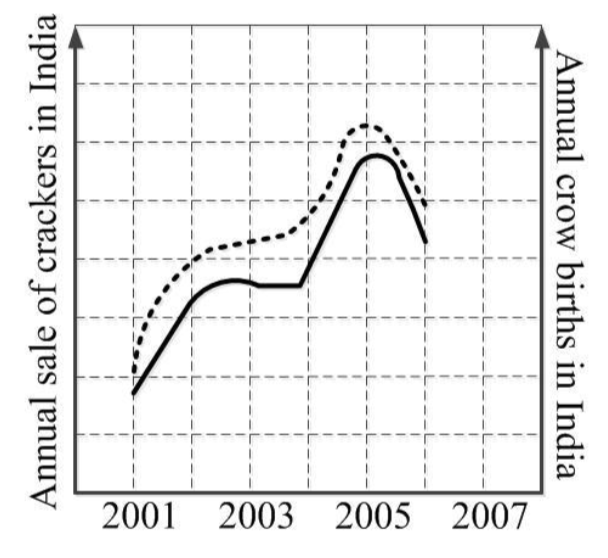
\includegraphics[width=0.7\columnwidth]{figs/10.png}
	\caption{}
	\label{fig10}
\end{center}
\end{figure}

\hfill \textbf{(GATE EE 2025)} \begin{enumerate}
    \item There is a strong correlation between cracker sales and crow births, so one must cause the other.
    \item The sale of crackers is a direct cause of the increase in crow births.
    \item The increase in crow population is a direct cause of the increase in cracker sales.
    \item There is a correlation between the two events, but no causal relationship can be inferred from the data.
\end{enumerate}


\begin{center}
\textbf{END OF THE QUESTION PAPER}
\end{center}
\newpage
 


{Q.1 - Q. 25 CARRY ONE MARK EACH.}

\item Consider the following two equations:
	\begin{align} \frac{dx}{dt}+x+y=0 \end{align}
		\begin{align} \frac{dy}{dt}-x=0 \end{align}
\normalsize The above set of equations is represented by
\hfill \textbf{(GATE EE 2025)} \begin{enumerate}
    \item $\dfrac{d^{2}y}{dt^{2}}-\dfrac{dy}{dt}-y=0$
    \item $\dfrac{d^{2}y}{dt^{2}}+\dfrac{dy}{dt}+y=0$
    \item $\dfrac{d^{2}y}{dt^{2}}-\dfrac{dy}{dt}+y=0$
    \item $\dfrac{d^{2}y}{dt^{2}}+\dfrac{dy}{dt}-y=0$
\end{enumerate}


\item The fourth order Runge-Kutta \brak{RK4} method to solve an ordinary differential equation
	\begin{align} \frac{dy}{dx}=f\brak{x,y} \end{align}
is given as \hfill \textbf{(GATE EE 2025)}
\begin{align*}
y\brak{x+h}&=y\brak{x}+\frac{1}{6}\brak{k_{1}+2k_{2}+2k_{3}+k_{4}} \\
k_{1}&=h~f\brak{x,y} \\
k_{2}&=h~f\brak{x+\frac{h}{2},y+\frac{k_{1}}{2}} \\
k_{3}&=h~f\brak{x+\frac{h}{2},y+\frac{k_{2}}{2}} \\
k_{4}&=h~f\brak{x+h,y+k_{3}}
\end{align*}
For a special case when the function $f$ depends solely on $x$, the above RK4 method reduces to
\hfill \textbf{(GATE EE 2025)} \begin{enumerate}
    \item Euler's explicit method
    \item Trapezoidal rule
    \item Euler's implicit method
    \item Simpson's $1/3$ rule
\end{enumerate}



\item A watch uses two electronic circuits \brak{ECs}. Each EC has a failure probability of 0.1 in one year of operation. Both ECs are required for functioning of the watch. The probability of the watch functioning for one year without failure is
\hfill \textbf{(GATE EE 2025)} \begin{enumerate}
    \item 0.99
    \item 0.90
    \item 0.81
    \item 0.80
\end{enumerate}


\newpage
The figure which represents $y=\frac{\sin x}{x}$ for $x>0$ $\brak{x}$ in radians is \hfill \textbf{(GATE EE 2025)}
\begin{figure}
\begin{center}
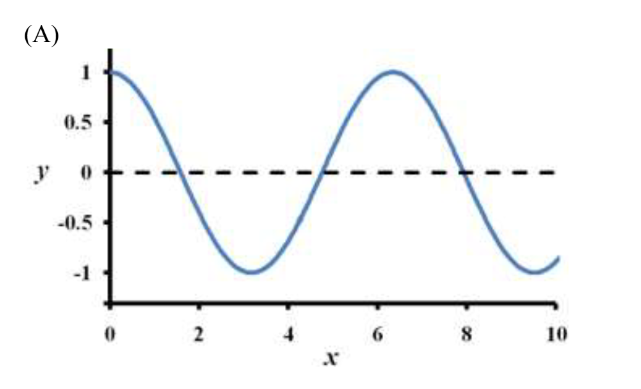
\includegraphics[width=0.7\columnwidth]{figs/4a.png}
	\caption{}
	\label{fig4a}
\end{center}
\end{figure}
\begin{figure}
\begin{center}
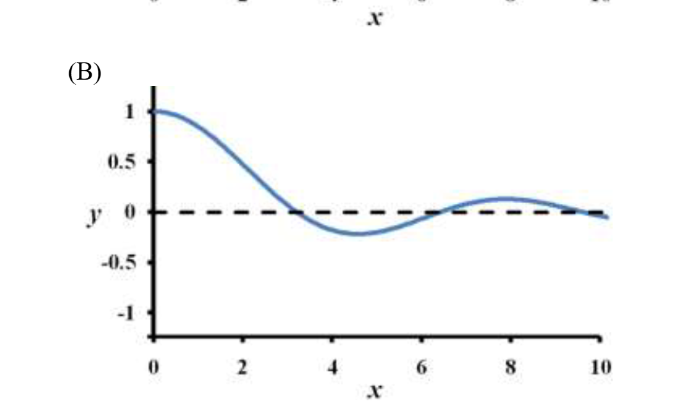
\includegraphics[width=0.7\columnwidth]{figs/4b.png}
	\caption{}
	\label{fig4b}
\end{center}
	\end{figure}
	\begin{figure}

\begin{center}
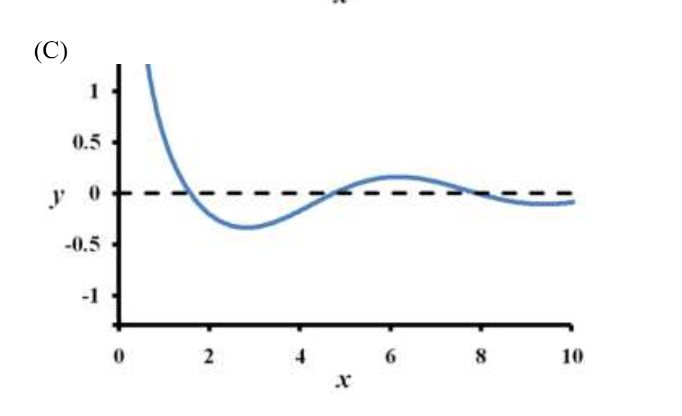
\includegraphics[width=0.7\columnwidth]{figs/4c.png}
	\caption{}
        \label{fig4c}
\end{center}
	\end{figure}
		\begin{figure}
\begin{center}
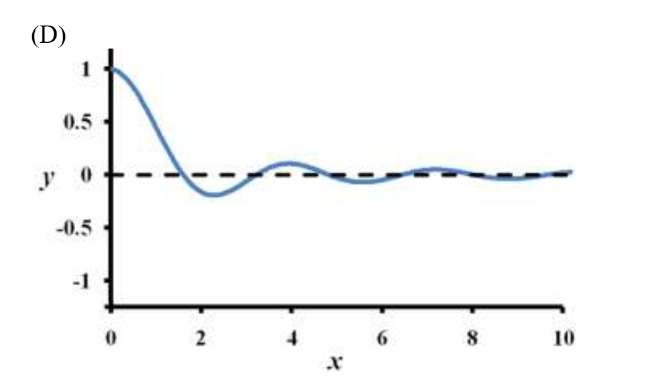
\includegraphics[width=0.7\columnwidth]{figs/4d.png}
  
\caption{}
\label{fig4d}
\end{center}
\end{figure}




\item The terminal velocity of a spherical particle in gravitational settling under Stokes' regime varies
\hfill \textbf{(GATE EE 2025)} \begin{enumerate}
    \item linearly with the particle diameter
    \item linearly with the viscosity of the liquid
    \item directly with the square of particle diameter
    \item inversely with the density of particle
\end{enumerate}
\textbf{$\brak{GATE EE 2025}$}

\item Critical speed of a ball mill depends on
\hfill \textbf{(GATE EE 2025)} \begin{enumerate}
    \item the radius of the mill \brak{shell} and the radius of the particles
    \item the radius of the mill \brak{shell} and the density of the particles
    \item the radius of the balls and the radius of the particles
    \item the radius of the balls and the radius of the mill \brak{shell}
\end{enumerate}


\item Economy of evaporators used for concentrating sugarcane juice is 
\hfill \textbf{(GATE EE 2025)} \begin{enumerate}
    \item $\dfrac{\text{kg of concentrated juice produced}}{\text{kg of steam supplied}}$
    \item $\dfrac{\text{kg of steam supplied}}{\text{kg of sugarcane juice fed}}$
    \item $\dfrac{\text{kg of water vaporized}}{\text{kg of steam supplied}}$
    \item $\dfrac{\text{kg of sugarcane juice fed}}{\text{kg of water vaporized}}$
\end{enumerate}

\item Segmental baffles in a 2-4 shell and tube heat exchanger
\hfill \textbf{(GATE EE 2025)} \begin{enumerate}
    \item change the flow pattern of the tube side fluid and increase the overall heat transfer co-efficient
    \item increase the heat transfer coefficient in the shell side and support the tubes
    \item help to reduce the thermal expansion of the tubes and increase the heat transfer coefficient in the tube side
    \item increase the number of passes in the shell side and increase the heat transfer coefficient in the tube side
\end{enumerate}


\item  In connection with petroleum refining, identify the incorrect statement among the following options.
\hfill \textbf{(GATE EE 2025)} \begin{enumerate}
    \item Desalting of crude oil is done before processing it in atmospheric distillation unit
    \item A stream of hydrogen is produced in catalytic reforming of naphtha
    \item Asphalt used for paving is a petroleum product
    \item Cetane number indicates the quality of petrol / motor spirit
\end{enumerate}


\item Polyvinyl chloride is produced by
\hfill \textbf{(GATE EE 2025)} \begin{enumerate}
    \item co-polymerization
    \item addition-type kinetics
    \item reacting chlorine with polyethylene
    \item reacting hydrochloric acid with polyethylene
\end{enumerate}
\hfill
\textbf{(GATE EE 2025)}

\item The molecular formula of the predominant chemical compound in commercial sugar is
\hfill \textbf{(GATE EE 2025)} \begin{enumerate}
    \item $C_{12}H_{22}O_{11}$
    \item $C_{12}H_{24}O_{12}$
    \item $C_{6}H_{10}O_{5}$
    \item $C_{6}H_{12}O_{6}$
\end{enumerate}


\item  Two packed towers are designed for the same mass velocity of the gas. The first has liquid and gas flow rates of 30 kg/s and 1.2 kg/s, respectively, while the corresponding flow rates in the second tower are $67.5~\text{kg/s}$ and $1.8~\text{kg/s}$. The ratio of the design diameter of the wider tower to that of the narrower tower is
\hfill \textbf{(GATE EE 2025)} \begin{enumerate}
    \item 2
    \item 1.8
    \item 1.5
    \item 1.225
\end{enumerate}

\item The Annual Fixed Charges \brak{AFC} and Annual Utilities Costs \brak{AUC} of a distillation column being designed are expressed in terms of the reflux ratio \brak{R} as
\[ \text{AFC \brak{Rs. Lakh}} = 641 R^{2}-1796 R+1287+1/\brak{R-1.16} \]
\[ \text{AUC \brak{Rs. Lakh}} = 80+62.5 R \]
The reflux ratio $\brak{R_{\text{opt}}}$ for optimizing the total cost of the distillation column may be found by solving
\hfill \textbf{(GATE EE 2025)} \begin{enumerate}
    \item $1282 R_{\text{opt}}-1796-1/\brak{R_{\text{opt}}-1.16}^{2}=0$
    \item $62.5+1282 R_{\text{opt}}-1796-1/\brak{R_{\text{opt}}-1.16}^{2}=0$
    \item $80+62.5 R_{\text{opt}}+641 R_{\text{opt}}^{2}-1796 R_{\text{opt}}+1287+1/\brak{R_{\text{opt}}-1.16}=0$
    \item $80+62.5 R_{\text{opt}}-641 R_{\text{opt}}^{2}+1796 R_{\text{opt}}-1287-1/\brak{R_{\text{opt}}-1.16}=0$
\end{enumerate}

\item Consider the following properties:
\brak{P} temperature
\brak{Q} specific gravity
\brak{R} chemical potential
\brak{S} volume
The option which lists ALL the intensive properties is
\hfill \textbf{(GATE EE 2025)} \begin{enumerate}
    \item P
    \item P and Q
    \item P, Q and R
    \item P, Q, R and S
	    
\end{enumerate}


\item  Liquid phase isomerization of o-xylene t
	o p-xylene using a zeolite catalyst was carried out in a CSTR. Three sets of kinetic data at different temperatures and stirring speeds were obtained as shown below.
	\begin{figure}
	\begin{center}
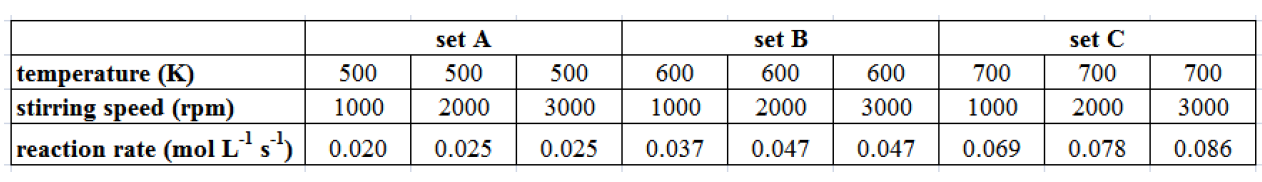
\includegraphics[width=1\columnwidth]{figs/16.png}
        \caption{}
	\label{fig16}
\end{center}
	\end{figure}
The operating condition at which the reaction rate is not controlled by external mass transfer resistance is
\hfill \textbf{(GATE EE 2025)} \begin{enumerate}
    \item $T=500~K$; rpm $=3000$
    \item $T=600~K$; rpm $=1000$
    \item $T=700~K$; rpm $=1000$
    \item $T=700~K$; rpm $=2000$
\end{enumerate}


\item Choose the correct statement. In viscose rayon manufacturing process,
\hfill \textbf{(GATE EE 2025)} \begin{enumerate}
    \item carbon disulphide used as reactant for xanthate formation is regenerated in a later step
    \item caustic soda used as reactant for steeping of cellulose is regenerated in a later step
    \item sulphuric acid is used in steeping process of cellulose
    \item the spun viscose rayon is hardened in an alkali bath
\end{enumerate}

<F20><F20><F20><F20><F20><F20><F20>
\item  The rea
ctant \brak{M}is converted into product \brak{N} in the presence of catalyst in a fixed bed reactor. All the flow rates \brak{F, G, H, P and R} in mol/s, and mole fraction of reactant \brak{M} in these streams $\brak{x_F, x_G, x_H, x_P \text{and} x_R}$ are shown in the diagram.
\begin{figure}
\begin{center}
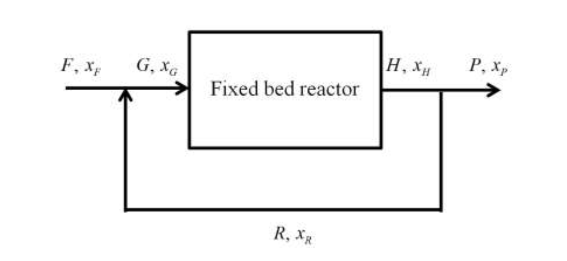
\includegraphics[width=0.7\columnwidth]{figs/17.png}
      \caption{}
      \label{fig17}
\end{center}
\end{figure}
The overall fractional conversion is
\hfill \textbf{(GATE EE 2025)} \begin{enumerate}
    \item $\dfrac{x_{G}G-x_{H}H}{x_{G}G}$
    \item $\dfrac{x_{G}G-x_{p}P}{x_{G}G}$
    \item $\dfrac{x_{F}F-x_{H}H}{x_{F}F}$
    \item $\dfrac{x_{F}F-x_{p}P}{x_{F}F}$
\end{enumerate}


\item A first-order process having a transfer function, $G_{p}=\dfrac{2}{7s+1}$, is controlled by a proportional controller with gain of 3.2. The process time constant is in minutes. Addition of the integral control action with an integral time constant of 5 minutes leads to increase in
\hfill \textbf{(GATE EE 2025)} \begin{enumerate}
    \item offset
    \item speed of response
    \item order of the closed loop system
    \item proportional band
\end{enumerate}


\item According to the surface renewal theory, the unit of fractional rate of surface renewal is
\hfill \textbf{(GATE EE 2025)} \begin{enumerate}
    \item $m^{2}s^{-2}$
    \item $m^{2}s^{-1}$
    \item $ms^{1}$
    \item $s^{-1}$
\end{enumerate}


\item For absorption of H$_2$S from a mixture with hydrocarbon vapour into an aqueous alkanolamine solution, the liquid phase mass transfer resistance is
\hfill \textbf{(GATE EE 2025)} \begin{enumerate}
    \item significantly higher than that of the gas phase
    \item negligible compared to that of the gas phase
    \item equal to that of the gas phase
    \item dependent on the gas phase mass transfer resistance
\end{enumerate}


\item  For a chemical reaction, the ratio of rate constant at 500 K to that at 400 K is 2.5. Given R $=8.314~\text{J mol}^{-1}\text{K}^{-1}$, the value of activation energy \brak{in kJ/mol} is
\hfill \textbf{(GATE EE 2025)} \begin{enumerate}
    \item 10.5
    \item 12.0
    \item 15.2
    \item 18.4
\end{enumerate}


\item  Pitot tube is used to measure
\hfill \textbf{(GATE EE 2025)} \begin{enumerate}
    \item liquid level in a tank
    \item flow velocity at a point
    \item angular deformation
    \item vorticity
\end{enumerate}


\item A venturi meter is installed to measure the flow rate of water in a 178 mm diameter \brak{ID} pipe. The throat diameter is 102 mm. The differential pressure measured using a manometer is $154.3~\text{kN/m}^{2}.$ The data given are: discharge coefficient $=0.98$; water density $=1000~\text{kg/m}^{3}$.
The volumetric flow rate of water $\brak{\text{in} \text{m}^{3}\text{/s}}$ is\underline{\hspace{2cm}}.\hfill \textbf{(GATE EE 2025)}

\item The ammonia $\brak{NH_{3}}$ oxidation process occurs over a catalyst as
\begin{align*}
    4\text{NH}_{3}+5\text{O}_{2}\rightarrow6\text{H}_{2}\text{O}+4\text{NO}
\end{align*}  
Air is supplied such that oxygen $\brak{O_2}$ is 20\% in excess of that required for complete conversion of NH$_3$. The mole fraction of O$_2$ in inlet gas mixture $\brak{NH_3 + \text{air}}$ is \_\_\_\_\_ (rounded off to third decimal place) \hfill \textbf{(GATE EE 2025)}.


\item  The initial water level in a tank is 4 m. When the valve located at the bottom is opened, the rate of change of water level \brak{L} with respect to time \brak{t} is $\frac{dL}{dt}=-k\sqrt{t}$, where $k=0.6~\text{m s}^{-3/2}$. The level of water \brak{in m} in the tank at time 0.5 s after opening the valve is\_\_\_\_\_ (rounded off to second decimal place)\hfill \textbf{(GATE EE 2025)}.


\textbf{Q.26 - Q. 55 CARRY TWO MARK EACH.}


\item  Match the equipment in Column A with the corresponding process in Column B
\begin{longtable}{|p{4cm}|p{6cm}|}
\hline
\textbf{Column A} & \textbf{Column B} \\
\hline
\brak{P} Centrifugal sifter & \brak{I} Mixing \\
\hline
\brak{Q} Bowl mill & \brak{II} Sedimentation \\
\hline
\brak{R} Gravity thickener & \brak{III} Screening \\
\hline
\brak{S} Two-arm kneader & \brak{IV} Grinding \\
\hline
\end{longtable}
\hfill \textbf{(GATE EE 2025)} \begin{enumerate}
    \item P-I, Q-IV, R-II, S-III
    \item P-III, Q-IV, R-II, S-I
    \item P-IV, Q-I, R-II, S-III
    \item P-IV, Q-III, R-I, S-II
\end{enumerate}


\item  In the year 2005, the cost of a shell and tube heat exchanger with $68~\text{m}^{2}$ heat transfer area was Rs. 12.6 Lakh. Chemical Engineering Index for cost in 2005 was 509.4 and now the index is 575.4. Based on index of 0.6 for capacity scaling, the present cost (in Lakhs of rupees) of a similar heat exchanger having $100~\text{m}^{2}$ heat transfer area is estimated to be
\hfill \textbf{(GATE EE 2025)} \begin{enumerate}
    \item 17.94
    \item 19.94
    \item 20.94
    \item 22.94
\end{enumerate}


\item A furnace installed at a cost of Rs. 24 Lakh is expected to serve its useful life of 5 years. Salvage value of the furnace is Rs. 8 Lakh. The interest rate compounded annually is 8\%. The estimated capitalized cost (in Lakhs of rupees) is
\hfill \textbf{(GATE EE 2025)} \begin{enumerate}
    \item 30
    \item 34.09
    \item 34.9
    \item 58.09
\end{enumerate}


\item G denotes the Gibbs free energy of a binary mixture, $n_T$ denotes the total number of moles present in the system, $\mu_{i}$ is the chemical potential of the $i^{th}$ component $\brak{\mu_{i}\ne0 \text{and} \mu_{1}>\mu_{2}}$ and $x_i$ is the mole fraction of the $i^{th}$ component. The correct variation of $G/n_{T}$ \brak{in J/mol} at constant temperature and pressure is given by \hfill \textbf{(GATE EE 2025)}
	\begin{figure}
\begin{center}
	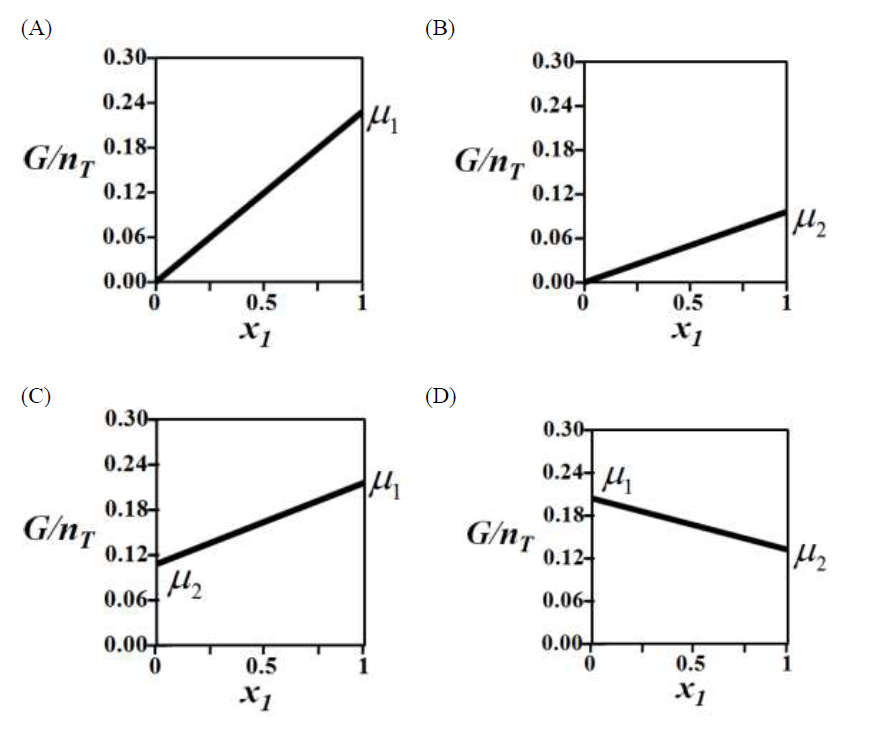
\includegraphics[width=0.7\columnwidth]{figs/29.png}
         \caption{}
	 \lable{fig29}
\end{center}
	\end{figure}
\item A person is drowning in sea at location R and the lifeguard is standing at location P. The beach boundary is straight and horizontal, as shown in the figure.\hfill \textbf{(GATE EE 2025)}
	\begin{figure}
\begin{center} 
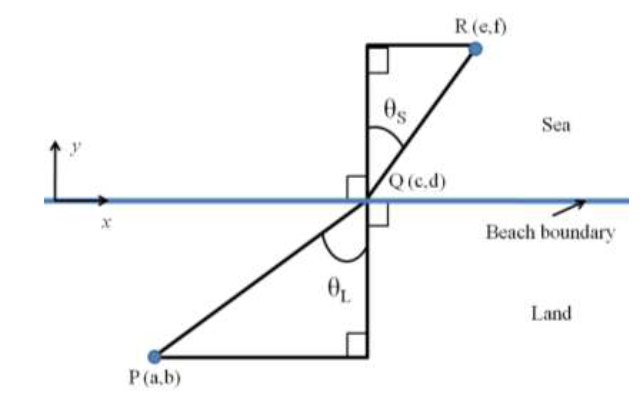
\includegraphics[width=0.7\columnwidth]{figs/30.png}
        \caption{}
	\label{fig30}
\end{center}
	\end{figure}
The lifeguard runs at a speed of $V_{L}$ and swims at a speed of $V_{S}$. In order to reach to the drowning person in optimum time, the lifeguard should choose point Q such that
\hfill \textbf{(GATE EE 2025)} \begin{enumerate}
    \item $\dfrac{\sin^{2}\theta_{L}}{\sin^{2}\theta_{S}}=\dfrac{V_{S}}{V_{L}}$
    \item $\dfrac{\sin\theta_{L}}{\sin\theta_{S}}=\dfrac{V_{S}}{V_{L}}$
    \item $\dfrac{\sin^{2}\theta_{L}}{\sin^{2}\theta_{S}}=\dfrac{V_{L}}{V_{S}}$
    \item $\dfrac{\sin\theta_{L}}{\sin\theta_{S}}=\dfrac{V_{L}}{V_{S}}$
\end{enumerate}
\item The decay ratio for a system having complex conjugate poles as $\brak{-\dfrac{1}{10}+j\dfrac{2}{15}}$ and $\brak{-\dfrac{1}{10}-j\dfrac{2}{15}}$ is
\hfill \textbf{(GATE EE 2025)} \begin{enumerate}
    \item $7\times10^{-1}$
    \item $8\times10^{-2}$
    \item $9\times10^{-3}$
    \item $10\times10^{-4}$
\end{enumerate}


\item Match the items in Column A with the items in Column B
\begin{longtable}{|p{4cm}|p{6cm}|}
\hline
\textbf{Column A} & \textbf{Column B} \\
\hline
\brak{P} Pure dead-time & \brak{I} $\phi=-90\degree$ \\
\hline
\brak{Q} Pure capacitive & \brak{II} $\dfrac{K_{1}}{s}-\dfrac{K_{2}}{\tau s+1}$ with $K_{2}>\tau K_{1}$ \\
\hline
\brak{R} Inverse response & \brak{III} $0<AR<1$ \\
\hline
\brak{S} First-order process with unit gain & \brak{IV} $AR=1$ \\
\hline
\end{longtable}
Here, $\phi$ denotes the phase shift, $K_{1}$ and $K_{2}$ the process gains, $\tau$ the time constant, and AR the amplitude ratio.
\hfill \textbf{(GATE EE 2025)} \begin{enumerate}
    \item P-II, Q-III, R-IV, S-I
    \item P-III, Q-II, R-IV, S-I
    \item P-I, Q-IV, R-II, S-III
    \item P-IV, Q-I, R-II, S-III
\end{enumerate}



\item In a laboratory batch setup, reaction of P over a catalyst was studied at various temperatures. The reactions occurring are
	\begin{align} P\rightarrow2Q \end{align}
		\begin{align} P\rightarrow R \end{align}
At the end of one hour of operation, the batch contains $x_{P}$, $x_{Q}$ and $x_{R}$ mole fractions of P, Q and R components, respectively. The mole fractions of product components $\brak{x_{Q} \text{and} x_{R}}$ were found to vary linearly with temperature as given in the figure. \hfill \textbf{(GATE EE 2025)}

\begin{figure}
	\begin{center}
  
 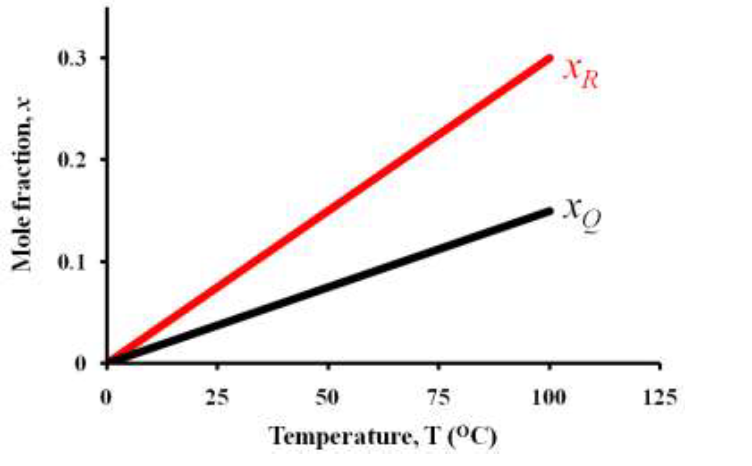
\includegraphics[width=0.7\columnwidth]{figs/33.png}
	\caption{}
	\label{fig33}
\end{center}
\end{figure}
If the yield of Q based on reactant P consumed $\brak{Y_{P}}$ at $25^{\circ}\text{C}$ was found to be 0.40, then the value of $Y_{P}$ at $60^{\circ}\text{C}$ is \_\_\_\_\_ (rounded off to second decimal place).\hfill \textbf{(GATE EE 2025)}

\item An insulated storage tank contains 1000 kg liquid of specific heat $10~\text{kJ kg}^{-1}\text{K}^{-1}$. The liquid is heated by saturated steam, condensing in a helical coil at a temperature of $180^{\circ}\text{C}$. The heat transfer area of the coil is $0.1~\text{m}^{2}$. If the overall heat transfer coefficient is constant at $1000~\text{W m}^{-2}\text{K}^{-1}$, then the time \brak{in hours} required to raise the temperature of the liquid in the tank from $20^{\circ}\text{C}$ to $80^{\circ}\text{C}$ is $\underline{\hspace{2cm}}$(rounded off to second decimal place). \hfill \textbf{(GATE EE 2025)}



\item The wall of a pipe of radius 1 m is at a uniform temperature of $200^{\circ}C$ and is covered by insulation of thickness 0.1 m. The ambient air outside the insulated pipe is at $20^{\circ}\text{C}$ and has heat transfer coefficient of $10~\text{W m}^{-2}\text{K}^{-1}$. The thermal conductivity of the insulation material is $0.05~{W m}^{-1}\text{K}^{-1}$. If the heat transfer occurs at steady state, the temperature $\brak{in {}^{\circ}\text{C}}$ of the outer surface of insulation is$\underline{\hspace{2cm}}$(rounded off to second decimal place).\hfill \textbf{(GATE EE 2025)}



\item  Vapour bubbles are formed in the nucleate boiling regime at a frequency of 10 bubbles per second per nucleation site. There are 100 nucleation sites per $m^2$ of heating area. The latent heat of vapourization and the density of vapour under the operating condition are $1000~\text{kJ/kg}$ and $1~\text{kg/m}^{3}$ respectively. The diameter of each bubble is $10^{-3}$ m. Assume that the entire heat supplied is used for vapour generation. The heat flux $\brak{\text{in Watt per} {m}^{2} \text{ of heating area}}$ is (rounded off to third decimal place).\hfill \textbf{(GATE EE 2025)}



\item Under isothermal condition, a vertical tube of length $L=100$ m contains a gas of molecular weight equal to 60. The pressure and temperature at the top of the tube are 100 kPa and $25^{\circ}\text{C}$ respectively. Consider the universal gas constant and acceleration due to gravity as $8.314~\text{J mol}^{-1}\text{K}^{-1}$ and $9.81~\text{m s}^{-2}$ respectively. If the gas is ideal, the pressure \brak{in kPa} at the bottom of the tube will be$\underline{\hspace{2cm}}$(rounded off to third decimal place). \hfill \textbf{(GATE EE 2025)} 



\item At a shear rate of $10~\text{s}^{-1}$, the apparent viscosity of a non-Newtonian liquid was found to be 1 Pa s. At a shear rate of $100~\text{s}^{-1}$, the apparent viscosity of the same liquid was found to be 0.5 Pa s. If the liquid follows power law behavior, the apparent viscosity \brak{in Pa s} at a shear stress of $10~\text{N m}^{-2}$ is$\underline{\hspace{2cm}}$(rounded off to two decimal place). \hfill \textbf{(GATE EE 2025)} 



 A CSTR and a PFR of equal volume are connected in series as shown below to carry out a first-order, isothermal, liquid phase reaction.
 \begin{figure}
\begin{center}
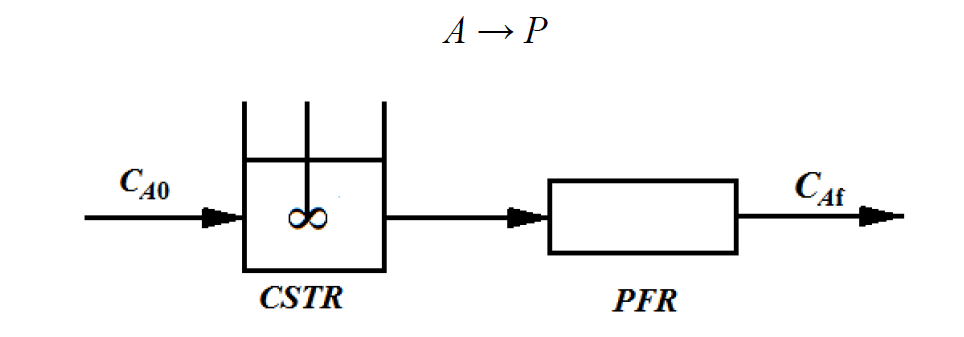
\includegraphics[width=0.8\columnwidth]{figs/39.png}
         \caption{}
	 \label{39}
\end{center}
 \end{figure}
The rate constant is $0.2~\text{s}^{-1}$. The space-time is 5 s for both the reactors. The overall fractional conversion of A is \_\_\_\_\_ (rounded off to third decimal place). \hfill \textbf{(GATE EE 2025)} 



\item  The elementary second-order liquid phase reaction $A+B\rightarrow C+D$ is carried out in an isothermal plug flow reactor of $2~\text{m}^{3}$ volume. The inlet volumetric flow rate is $10~\text{m}^{3}/\text{h}$. The initial concentrations of both A and B are $2~\text{kmol/m}^{3}$. The rate constant is given as $2.5~\text{m}^{3} \text{kmol}^{-1} \text{h}^{-1}$. The percentage conversion of A is\_\_\_\_\_\_\_\_\_\_.




\item It is decided to extract A from a feed containing 20 mol\% A and 80 mol\% B in two ideal cross-current stages as shown below, using equal amount of pure solvent C in each stage.
	\begin{figure}
\begin{center}
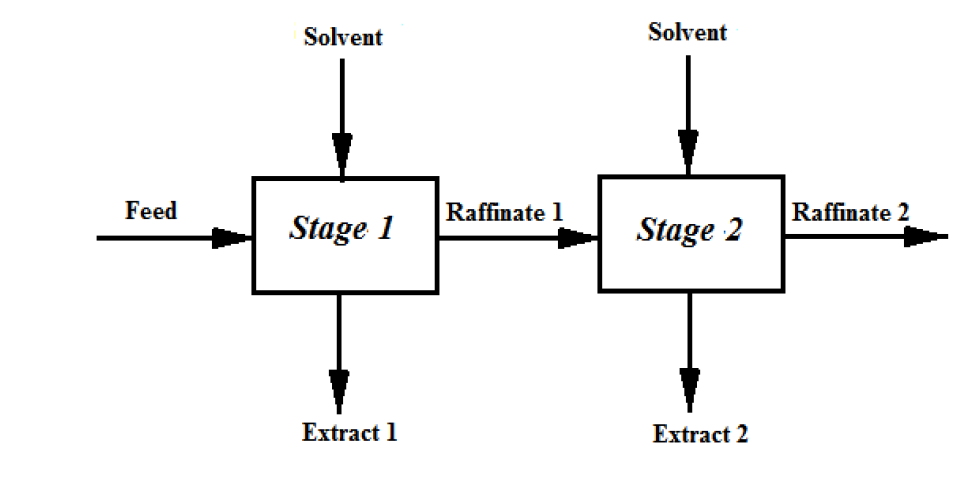
\includegraphics[width=0.8\columnwidth]{figs/41.png}
     \caption{}
      \ label{fig41}
\end{center}
	\end{figure}
Components B and C are immiscible. 60\% of A in the feed is extracted in Stage 1. The equilibrium relation is given by $Y^{*}=1.5 X$ where, \\
$X=$ moles of A per mole of B in raffinate \\
$Y^{*}=$ moles of A per mole of C in extract in equilibrium with raffinate
\\
The mol\% of A in raffinate from Stage 2 is$\underline{\hspace{2cm}}$(rounded off to second decimal place). \hfill \textbf{(GATE EE 2025)} 



\item A binary distillation column is designed by McCabe-Thiele method to get a distillate mole fraction of 0.9. The enriching section operating line has an intercept with y-axis at 0.3 mole fraction. The ratio of liquid to vapour molar flow rate in the enriching section is$\underline{\hspace{2cm}}$(rounded off to third decimal place). \hfill \textbf{(GATE EE 2025)} 



\item A fiberboard sheet $\brak{1.5~\text{m}\times2.0~\text{m}\times15~\text{mm}}$ is being dried by suspending it horizontally in a current of hot, dry air. The edges are insulated so that drying takes place only from the top and bottom surfaces. The wet sheet weighing 16 kg with initial moisture content of 60\% loses moisture at a constant rate of $1.25\times10^{-5}~\text{kg m}^{-2}\text{s}^{-1}$ until the moisture content falls to 30\%. All moisture contents are on dry basis. The time required for drying during constant rate period \brak{in hour} is$\underline{\hspace{2cm}}$(rounded off to third decimal place). \hfill \textbf{(GATE EE 2025)} 



\item Consider the following transfer function:
	\begin{align} G\brak{s}=\frac{3}{\brak{5s+1}^{2}} \end{align}
where, the natural period of oscillation is in min. The amplitude ratio at a frequency of 0.5 rad/min is$\underline{\hspace{2cm}}$(rounded off to second decimal place). \hfill \textbf{(GATE EE 2025)} 


\item For a closed-loop system, consider the following transfer functions:
process $G_{p}\brak{s}$, controller $G_{c}\brak{s}$, measuring device $G_{m}\brak{s},$ and final control element $G_{f}\brak{s}$
\begin{align} G_{p}\brak{s} = \frac{2}{7s+1}
\G_{c}\brak{s}=2 
\G_{m}\brak{s}=1 
\G_{f}\brak{s}=1 \end{align}
The offset in the closed loop response due to a unit step change introduced in the set point of the output variable is\_\_\_\_\_\_\_\_\_\_.




\item If $y=e^{-x^{2}}$, then the value of $\lim_{x\rightarrow\infty}\frac{1}{x}\frac{dy}{dx}$ is\_\_\_\_\_\_\_\_\_\_.



\item For the matrix $A = \begin{pmatrix} \cos\theta & -\sin\theta \\ \sin\theta & \cos\theta \end{pmatrix}$, if det stands for the determinant and $A^{T}$ is the transpose of A then the value of $\det\brak{A^{T}A}$ is \_\_\_\_\_\_\_\_\_\_.



\item An azeotropic mixture of ethanol and water is to be separated in a distillation column using benzene as an entrainer. At the column operating conditions, two liquid phases are formed on a tray. The degree\brak{s} of freedom of the system for the choice of intensive properties at equilibrium is\brak{are} \_\_\_\_\_\_\_\_\_\_.




\item The volume of liquid filled in a spherical storage tank of radius R is computed from height of liquid, h, in the outside tube (neglecting the volume of liquid in the outside tube) as
\[ V=\pi h^{2}\frac{\brak{3R-h}}{3} \]
\begin{figure}
\begin{center}
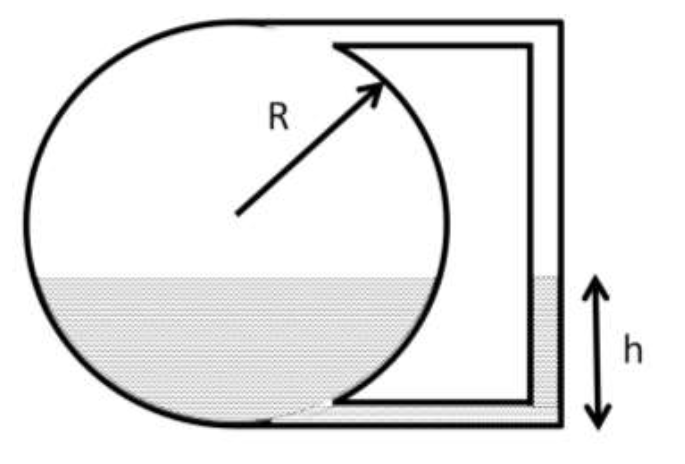
\includegraphics[width=0.3\columnwidth]{figs/49.png}
     \caption{}
     \label{fig49}

\end{center}
\end{figure}
The estimate of liquid height \brak{in m} to store $V=30~\text{m}^{3}$ of water in a $R=3$ m tank, after performing ONE iteration of Secant method, using 1 m and 3 m as two initial guesses of liquid height is$\underline{\hspace{2cm}}$(rounded off to second decimal place). \hfill \textbf{(GATE EE 2025)} 



\item In a closed piston-cylinder system, methane was observed to obey the following equation of state
\[ P\brak{V-nb}=nRT \]
where $b=0.029~\text{m}^{3}/\text{mol}$. The temperature and volume are $500^{\circ}\text{C}$ and $5\text{m}^{3}$ respectively for 100 moles of methane. At this state of the system, the isobaric rate of change of temperature with volume $\brak{in ^{\circ}\text{C/m}^{3}}$ is\underline{\hspace{2cm}} (rounded off to second decimal place).



\item A set of standard stainless steel pipes, each of internal diameter 26.65 mm and 6000 mm length, is used to make a plug flow reactor by joining them in series to carry out degradation of polyethylene. Seven such pipes are required to obtain a conversion of 66\% at 450 K. The minimum number of standard 8000 mm long pipes of the same internal diameter to be procured for obtaining at least 66\% conversion under the same reaction conditions is\_\_\_\_\_\_\_\_\_\_.\hfill \textbf{(GATE EE 2025)} 




\item Hydrogenation of benzene is to be carried out using Ni $\brak{\text{density} = 8910~\text{kg/m}^{3}}$ as catalyst, cast in the form of non-porous hollow cylinders, as shown below. The reaction occurs on all the surfaces of the hollow cylinder. During an experiment, one such cylinder is suspended in the reactant stream. If the observed rate of reaction is $0.39~\text{mol}\cdot\brak{\text{m}^2 \text{ of catalyst surface}}^{-1}\cdot\text{min}^{-1}$, then the rate of reaction in $\text{mol}\cdot\brak{\text{kg of catalyst}}^{-1}\cdot\text{min}^{-1}$ is\underline{\hspace{2cm}} (rounded off to three decimal places). \hfill \textbf{(GATE EE 2025)} 
	\begin{figure}

\begin{center}
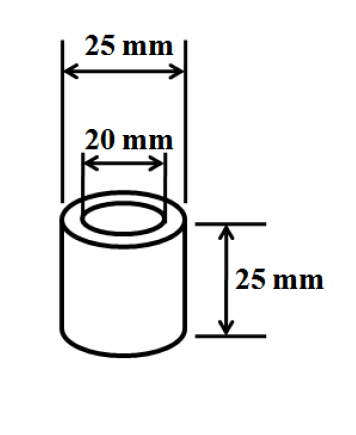
\includegraphics[width=0.2\columnwidth]{figs/52.png}
      \caption{}
      \label{fig52}
	\end{center}
	\end{figure}


\item The humidity of air at a dry-bulb temperature of $65^{\circ}\text{C}$ is 0.025 kg water/kg dry air. The latent heat of vaporization of water at $0^{\circ}\text{C}$ is $2500~\text{kJ/kg}$. The psychrometric ratio of air is $0.95~\text{kJ \brak{kg dry air}}^{-1}\text{K}^{-1}$. Considering $0^{\circ}\text{C}$ as reference temperature, the enthalpy of air \brak{in kJ/kg} at its adiabatic saturation temperature of $35^{\circ}\text{C}$ is$\underline{\hspace{2cm}}$(rounded off to two decimal places).\hfill \textbf{(GATE EE 2025)} 



\item  In a roll crusher, rolls of diameter 1 m each are set in such a manner that minimum clearance between the crushing surfaces is 15 mm. If the angle of nip is $31^{\circ}$, the maximum diameter of the particle  (in mm) which can be crushed is $\underline{\hspace{2cm}}$ (rounded off to third decimal place).
\hfill \textbf{(GATE EE 2025)} 

\item A hot liquid is to be cooled in a 1-1 shell and tube heat exchanger from $80^{\circ}\text{C}$ to $50^{\circ}\text{C}$. Cooling water enters the tube side at $30^{\circ}\text{C}$ and exits at $45^{\circ}\text{C}$. The properties of the liquids are constant. Also, the overall heat transfer coefficient is same for counter-current and co-current modes. The percentage saving in heat transfer xarea for counter-current option with respect to the area of co-current option is$\underline{\hspace{2cm}}$ (rounded off to third decimal place).  \hfill \textbf{(GATE EE 2025)} 


\end{enumerate}

\end{document}
